\documentclass[journal, a4paper, twocolumn]{IEEEtran}

% ======================================================
% PACKAGES ESSENTIELS
% ======================================================
\usepackage[utf8]{inputenc}
\usepackage[T1]{fontenc}
\usepackage[french]{babel}
\usepackage{graphicx}
\usepackage{amsmath, amssymb, amsfonts}
\DeclareMathOperator*{\argmin}{arg\,min}  % operateur argmin
\usepackage{bm}          % Vecteurs en gras dans les équations
\usepackage{booktabs}    % Tableaux professionnels
\usepackage{hyperref}
\usepackage{xcolor}
\usepackage{listings}
\usepackage{float}
\usepackage{enumitem}
\usepackage{tikz}        % Schémas TikZ (si disponible)
\usepackage{caption}
\usepackage{subcaption}

% ======================================================
% CONFIGURATION DU STYLE DES BLOCS DE CODE (lstlistings)
% ======================================================
\definecolor{codegreen}{rgb}{0,0.6,0}
\definecolor{codegray}{rgb}{0.5,0.5,0.5}
\definecolor{codepurple}{rgb}{0.58,0,0.82}
\definecolor{backcolour}{rgb}{0.95,0.95,0.92}
\definecolor{keyblue}{rgb}{0.0,0.3,0.7}

\lstdefinestyle{pythonstyle}{
    backgroundcolor=\color{backcolour},
    commentstyle=\color{codegreen}\itshape,
    keywordstyle=\color{keyblue}\bfseries,
    numberstyle=\tiny\color{codegray},
    stringstyle=\color{codepurple},
    basicstyle=\ttfamily\scriptsize,
    breakatwhitespace=false,
    breaklines=true,
    captionpos=b,
    keepspaces=true,
    numbers=left,
    numbersep=5pt,
    showspaces=false,
    showstringspaces=false,
    showtabs=false,
    tabsize=2,
    frame=single,
    rulecolor=\color{codegray}
}
\lstset{style=pythonstyle}

% ======================================================
% PAGE DE TITRE
% ======================================================
\title{\textbf{STHENOS} --- Métamodélisation par Intelligence Artificielle pour la substitution d'un solveur par éléments finis en mécanique des structures}

\author{Rayan Chennaoui, Nima Kashani~\IEEEmembership{Étudiants IPSA 4A},\\
        Spécialité Mécanique / Structures Aéronautiques\\
        \texttt{rayan.chennaoui@ipsa.fr, nima.kashani@ipsa.fr}}

\begin{document}

\maketitle

% ======================================================
% ABSTRACT (Français)
% ======================================================
\noindent\textbf{STHENOS} (du grec ancien $\Sigma\theta\acute{\epsilon}\nu o\varsigma$, signifiant \textit{la force}, \textit{la puissance}).

\begin{abstract}
L'analyse par éléments finis (FEA) est un pilier du dimensionnement structural en aéronautique, mais son coût computationnel prohibitif limite son intégration dans les boucles d'optimisation itérative. Le projet \textbf{STHENOS} détaille la création d'un métamodèle basé sur l'Intelligence Artificielle (\textit{Surrogate Model}) pour remplacer le solveur MSC Nastran (SOL 101) dans l'étude d'une poutre 3D encastrée-libre maillée en éléments volumiques HEXA20. En s'appuyant sur un plan d'expériences généré par \textit{Latin Hypercube Sampling} (LHS) sur deux paramètres ($L \in [500,2500]$ mm, $F \in [1000,16000]$ N), un jeu de données de 296 points a été constitué via un pipeline automatisé de génération de fichiers \texttt{.bdf}, d'exécution Nastran en mode batch et de parsing des fichiers \texttt{.f06} par expressions régulières. Trois architectures de Machine Learning ont été développées avec la bibliothèque scikit-learn : Régression Polynomiale avec régularisation Ridge, Forêt Aléatoire et Réseau de Neurones Multi-Couches (MLP). Le MLP surpasse les autres modèles avec un coefficient de détermination $R^2 > 0.999$, une erreur absolue moyenne MAE $\approx 3$ mm sur la flèche et $\approx 6.4$ MPa sur la contrainte de Von Mises, le tout pour un facteur de gain de vitesse (\textit{Speed-Up}) de $\mathbf{\times 50\,000}$ par rapport au solveur EF. Un démonstrateur temps réel est déployé sous Streamlit.
\end{abstract}

% ======================================================
% ABSTRACT (Anglais)
% ======================================================
\textbf{\textit{Abstract}---Finite Element Analysis (FEA) is a cornerstone of structural sizing in aeronautics, but its prohibitive computational cost limits its integration into iterative optimization loops. The \textbf{STHENOS} project details the creation of an AI-based surrogate model to replace the MSC Nastran solver (SOL 101) in the study of a 3D cantilever beam meshed with HEXA20 volumetric elements. Based on a Design of Experiments generated by Latin Hypercube Sampling (LHS) over two parameters ($L \in [500,2500]$ mm, $F \in [1000,16000]$ N), a dataset of 296 points was built via an automated pipeline for \texttt{.bdf} generation, batch Nastran execution, and \texttt{.f06} parsing via regular expressions. Three Machine Learning architectures were developed using scikit-learn: Polynomial Ridge Regression, Random Forest, and Multi-Layer Perceptron (MLP). The MLP achieves $R^2 > 0.999$, MAE $\approx 3$ mm and $\approx 6.4$ MPa, with a Speed-Up factor of $\mathbf{\times 50,000}$ over FEA. A real-time demonstrator is deployed with Streamlit.}

% ======================================================
% SECTION 1 : INTRODUCTION ET CONTEXTE AERONAUTIQUE
% ======================================================
\section{Introduction \& Contexte Aéronautique}

\subsection{Le défi du dimensionnement structural}
Le dimensionnement structural est le processus par lequel l'ingénieur aéronautique s'assure qu'une pièce --- aile, fuselage, longeron, cadre --- résiste aux chargements auxquels elle sera soumise en vol, au décollage, à l'atterrissage, etc. Pour ce faire, il doit connaître, pour chaque point du solide, les \textbf{contraintes mécaniques} (les forces internes par unité de surface, en Pa ou MPa) et les \textbf{déplacements} (la déformation de la structure, en mm).

Pendant des décennies, cette tâche s'est appuyée exclusivement sur des formules analytiques issues de la résistance des matériaux (RDM) et de la théorie des plaques. Mais ces formules, aussi élégantes soient-elles, ne valent que pour des géométries simples : une poutre droite à section constante, une plaque mince, une coque cylindrique.

Un avion moderne, en revanche, présente des géométries d'une complexité extraordinaire. La seule approche universellement applicable est la \textbf{Méthode des Éléments Finis} (MEF ou FEA), implémentée dans des codes comme MSC Nastran, Abaqus ou ANSYS.

\subsection{Le coût prohibitif de la MEF}
La MEF discrétise le domaine continu d'un solide en milliers, voire en millions de petits blocs appelés \textbf{éléments}. Chaque nœud connectant ces éléments se voit attribuer des inconnues (déplacements), et les équations de la physique permettent d'écrire un gigantesque système linéaire $[K]\{U\} = \{F\}$. La résolution de ce système est l'opération fondamentale, et son coût est de l'ordre $\mathcal{O}(n^3)$ où $n$ est le nombre de degrés de liberté.

Pour un modèle d'avion complet comportant plusieurs millions de nœuds, chaque résolution peut prendre de plusieurs minutes à plusieurs heures. Dans un processus d'optimisation de forme ou de topologie, ce solveur peut être appelé des milliers de fois. Il devient alors un \textbf{verrou computationnel}.

\subsection{La solution : les Surrogate Models}
L'idée du \textit{Surrogate Model} (ou métamodèle) est de remplacer ce solveur coûteux par une fonction mathématique apprise sur un ensemble d'exemples préalablement calculés. Cette approche ne repose plus sur la physique interne du solveur, mais sur la reconnaissance de patterns dans les données.

Le présent projet constitue une implémentation de bout en bout de cette philosophie, de la génération des données Nastran jusqu'au déploiement d'une interface web interactive.

% ======================================================
% SECTION 2 : MECANIQUE DES MILIEUX CONTINUS (MMC)
% ======================================================
\section{Rappels de Mécanique des Milieux Continus}
\label{sec:mmc}

Cette section est un préambule théorique indispensable. Elle pose les fondements de la physique que notre IA devra imiter.

\subsection{Qu'est-ce qu'un milieu continu ?}

Un \textbf{milieu continu} est une idéalisation mathématique de la matière. Au lieu de modéliser chaque atome ou molécule individuellement, on suppose que la matière est répartie de manière continue dans l'espace. Cette hypothèse est valide dès lors que l'échelle d'observation est grande devant l'échelle moléculaire, ce qui est le cas en mécanique des structures (où l'on parle de millimètres à mètres).

\subsection{Le tenseur des contraintes}

Lorsqu'un solide est soumis à des forces, des efforts internes apparaissent. Pour les caractériser, on coupe mentalement le solide par un plan et on regarde les forces que la partie gauche exerce sur la partie droite.

Ces forces internes s'expriment par unité de surface et définissent le \textbf{vecteur-contrainte} $\bm{T}$. Sa décomposition dans le repère cartésien $(x, y, z)$ fait intervenir 9 composantes, regroupées dans le \textbf{tenseur de Cauchy des contraintes} :
\begin{equation}
    [\bm{\sigma}] = \begin{pmatrix}
    \sigma_{xx} & \sigma_{xy} & \sigma_{xz} \\
    \sigma_{yx} & \sigma_{yy} & \sigma_{yz} \\
    \sigma_{zx} & \sigma_{zy} & \sigma_{zz}
    \end{pmatrix}
\end{equation}
Les termes diagonaux ($\sigma_{xx}, \sigma_{yy}, \sigma_{zz}$) sont les \textbf{contraintes normales} (traction/compression). Les termes hors-diagonaux ($\sigma_{xy}$, etc.) sont les \textbf{contraintes de cisaillement}. Par symétrie du tenseur ($\sigma_{ij} = \sigma_{ji}$), seules 6 composantes sont indépendantes.

\subsection{La contrainte de Von Mises $\sigma_{VM}$}

Comparer un état de contrainte complexe (avec normales et cisaillements) à la limite élastique d'un matériau testée en traction simple est un problème non trivial. Le critère de \textbf{Von Mises} (1913) fournit une réponse élégante : il définit une contrainte équivalente scalaire $\sigma_{VM}$ à partir du déviateur du tenseur des contraintes.

En termes de contraintes principales $\sigma_1, \sigma_2, \sigma_3$ :
\begin{equation}
    \sigma_{VM} = \sqrt{\frac{(\sigma_1-\sigma_2)^2 + (\sigma_2-\sigma_3)^2 + (\sigma_3-\sigma_1)^2}{2}}
\end{equation}
La condition de rupture plastique est simplement $\sigma_{VM} \geq \sigma_e$ où $\sigma_e$ est la limite élastique du matériau. C'est \textbf{cette grandeur} que Nastran calcule et que notre IA apprend à prédire.

\subsection{Le tenseur des déformations}

Sous l'effet des contraintes, le solide se déforme. La déformation locale est quantifiée par le \textbf{tenseur des petites déformations} $\bm{\varepsilon}$, défini à partir du champ de déplacement $\bm{u}(x,y,z)$ par :
\begin{equation}
    \varepsilon_{ij} = \frac{1}{2}\left(\frac{\partial u_i}{\partial x_j} + \frac{\partial u_j}{\partial x_i}\right)
\end{equation}
Les composantes diagonales $\varepsilon_{ii}$ représentent les allongements relatifs (dilatations), et les composantes hors-diagonale les glissements angulaires.

\subsection{La loi de Hooke généralisée (comportement élastique)}

Pour un matériau élastique linéaire et isotrope (hypothèse valide pour les métaux en petites déformations), la relation entre contraintes et déformations est la \textbf{loi de Hooke généralisée} :
\begin{equation}
    \sigma_{ij} = \lambda \, \varepsilon_{kk} \, \delta_{ij} + 2\mu \, \varepsilon_{ij}
\end{equation}
où $\lambda$ et $\mu$ sont les \textbf{coefficients de Lamé} liés au module de Young $E$ et au coefficient de Poisson $\nu$ par :
\begin{equation}
    \lambda = \frac{E\nu}{(1+\nu)(1-2\nu)}, \quad \mu = \frac{E}{2(1+\nu)}
\end{equation}
C'est l'équation constitutive du matériau. Elle ferme le système d'équations de la MMC.

\subsection{Les équations d'équilibre de Navier}

En combinant la loi de Hooke, la définition des déformations et les équations d'équilibre local ($\nabla \cdot \bm{\sigma} + \bm{f} = \bm{0}$), on obtient les \textbf{équations de Navier} qui gouvernent le champ de déplacement $\bm{u}$ :
\begin{equation}
    (\lambda + \mu)\,\nabla(\nabla \cdot \bm{u}) + \mu\,\nabla^2 \bm{u} + \bm{f} = \bm{0}
\end{equation}
C'est ce système d'équations aux dérivées partielles (EDP), couplé à des conditions aux limites (encastrement, forces appliquées), que la MEF résout numériquement.

% ======================================================
% SECTION 3 : THÉORIE DES POUTRES ET MODÈLE EF
% ======================================================
\section{Modèle Physique : Poutre d'Euler-Bernoulli et HEXA20}

\subsection{La théorie des poutres d'Euler-Bernoulli}

La théorie des poutres d'Euler-Bernoulli (EBT) est une simplification 1D des équations de Navier, valable lorsque la longueur $L$ est grande devant les dimensions de la section transversale. Ses hypothèses sont :
\begin{enumerate}[label=\textbf{H\arabic*}.]
    \item Les sections droites restent planes et perpendiculaires à la fibre neutre après déformation.
    \item Les déformations sont de petite amplitude.
    \item Le matériau est élastique, linéaire, et isotrope.
\end{enumerate}

Sous ces hypothèses, et pour une poutre encastrée à une extrémité ($x=0$) et soumise à une force concentrée $F$ à l'autre ($x=L$), on peut dériver analytiquement les équations suivantes.

L'équation différentielle de la déformée $v(x)$ est :
\begin{equation}
    EI \frac{d^4 v}{dx^4} = q(x)
\end{equation}
Pour un effort ponctuel $F$ en bout, $q(x)=0$ sur $[0,L[$ et l'intégration directe donne le profil :
\begin{equation}
    v(x) = \frac{F}{6EI}\left(3Lx^2 - x^3\right)
\end{equation}

La \textbf{flèche maximale} à l'extrémité libre ($x=L$) est donc :
\begin{equation}
    \boxed{\delta_{\max} = \frac{F L^3}{3EI}}
    \label{eq:fleche}
\end{equation}

Le moment fléchissant $M_f(x) = F(L-x)$ est maximal en pied d'encastrement ($x=0$). La \textbf{contrainte maximale de flexion} (en surface, à distance $h/2$ de la fibre neutre) est :
\begin{equation}
    \boxed{\sigma_{\max} = \frac{M_{f,\max} \cdot (h/2)}{I_z} = \frac{F \cdot L \cdot (h/2)}{I_z}}
    \label{eq:sigma}
\end{equation}
où $I_z = bh^3/12$ est le moment d'inertie de la section rectangulaire de largeur $b$ et hauteur $h$.

\subsection{Limites de la théorie EBT et passage au modèle 3D HEXA20}

Les équations~\eqref{eq:fleche} et~\eqref{eq:sigma} sont remarquablement simples, mais elles ignorent des phénomènes réels importants :
\begin{itemize}
    \item Le cisaillement transversal (non pris en compte par l'hypothèse H1).
    \item Les effets de concentration de contraintes à l'encastrement.
    \item Le gauchissement des sections.
\end{itemize}

Pour capturer ces effets, notre modèle Nastran utilise des éléments \textbf{HEXA20} : des hexaèdres à 20 nœuds (8 nœuds de coin + 12 nœuds de milieu d'arête). Ces éléments d'ordre 2 permettent de représenter des champs de déplacement quadratiques à l'intérieur de chaque élément, offrant une précision nettement supérieure aux éléments linéaires HEXA8. Le format Nastran \texttt{.bdf} décrit ce maillage sous la forme de cartes \texttt{GRID} (coordonnées nodales) et \texttt{CHEXA} (connectivités).

\subsection{L'équation matricielle globale de la MEF}

L'essence de la MEF est d'assembler les matrices de rigidité élémentaires $[k_e]$ de chaque élément pour former la matrice de rigidité globale $[K]$. La résolution du système global donne les déplacements nodaux, puis par post-traitement les contraintes sont calculées.

\begin{equation}
    [K] = \sum_e [T_e]^T [k_e] [T_e], \quad [K]\{U\} = \{F\}
\end{equation}

La matrice élémentaire d'un HEXA20 est construite par intégration numérique de Gauss sur 27 points d'intégration :
\begin{equation}
    [k_e] = \int_V [B]^T [D] [B] \, dV \approx \sum_{i=1}^{27} w_i [B(\xi_i)]^T [D] [B(\xi_i)] |\det J(\xi_i)|
\end{equation}
où $[B]$ est la matrice des dérivées des fonctions de forme (opérateur cinématique) et $[D]$ est la matrice de comportement constitutive du matériau (issue de la loi de Hooke généralisée).

% ======================================================
% SECTION 4 : ETAT DE L'ART
% ======================================================
\section{État de l'Art : Du Solveur EF aux Surrogate Models}

\subsection{La révolution Data-Driven Engineering}

L'émergence du \textit{Machine Learning} dans les sciences de l'ingénieur au cours de la dernière décennie a ouvert une voie nouvelle : plutôt que de résoudre les équations de la physique, on apprend la relation entrée-sortie à partir d'exemples. Cette approche, regroupée sous l'appellation \textit{Data-Driven Engineering}, complète (et parfois remplace) les méthodes classiques.

Les métamodèles les plus répandus en mécanique des structures sont :
\begin{itemize}
    \item \textbf{Krigeage (GPR)} : Interpolation bayésienne, offre des estimations d'incertitude. Très performant en faibles dimensions.
    \item \textbf{Machines à Vecteurs de Support (SVM)} : Robuste avec peu de données, mais peu scalable.
    \item \textbf{Réseaux de Neurones (MLP, CNN)} : Scalables, capables de capturer des non-linéarités complexes, actuellement à l'état de l'art.
    \item \textbf{Physics-Informed Neural Networks (PINNs)} : Intègrent les équations de Navier directement dans la fonction de coût. Perspective d'avenir du projet STHENOS.
\end{itemize}

% ======================================================
% SECTION 5 : MÉTHODOLOGIE ET PLAN D'EXPÉRIENCES
% ======================================================
\section{Méthodologie et Plan d'Expériences (DoE)}

\subsection{Définition du domaine paramétrique}

Notre système comporte deux paramètres de conception libres :
\begin{itemize}
    \item La longueur de la poutre : $L \in [500, 2500]$ mm.
    \item La force appliquée : $F \in [1000, 16000]$ N.
\end{itemize}
Tous les autres paramètres (section transversale $b \times h = 50 \times 50$ mm, matériau aluminium $E = 70$ GPa, $\nu = 0.3$) sont maintenus constants.

\subsection{L'échantillonnage de Monte Carlo (référence)}

L'approche la plus naïve pour explorer un espace de paramètres est le \textbf{tirage aléatoire de Monte Carlo (MC)} : on tire $N$ points indépendamment et uniformément dans chaque dimension. Soit $X_j \sim \mathcal{U}(a_j, b_j)$ pour la variable $j$, le point $i$ du plan MC est :
\begin{equation}
    X_i^j = a_j + (b_j - a_j) \cdot U_{ij}, \quad U_{ij} \sim \mathcal{U}(0,1)
\end{equation}
Le problème de MC est sa convergence lente et l'apparition de zones sur- ou sous-peuplées dans l'espace des paramètres (\textit{clustering} et \textit{gaps}). Pour $N$ points en dimension $d$, la variance de l'estimateur MC est en $\mathcal{O}(N^{-1})$, indépendamment de $d$. Ce "fléau de la dimensionnalité" est toléré en grande dimension, mais en dimension 2 on peut faire bien mieux.

\subsection{Le Latin Hypercube Sampling (LHS)}

Le \textbf{LHS} (McKay, Beckman, Conover, 1979) est une méthode de quasi-Monte Carlo qui garantit une couverture stratifiée et optimale de l'espace des paramètres.

\textbf{Principe algorithmique :}
\begin{enumerate}
    \item Diviser chaque dimension en $N$ intervalles équiprobables : $[0, 1/N[$, $[1/N, 2/N[$, ..., $[(N-1)/N, 1]$.
    \item Pour chaque dimension $j$, générer une permutation aléatoire $\pi_j$ des entiers $\{1, \ldots, N\}$.
    \item L'échantillon normalisé $i$ dans la dimension $j$ est :
    \begin{equation}
        \tilde{X}_i^j = \frac{\pi_j(i) - U_{ij}}{N}, \quad U_{ij} \sim \mathcal{U}(0,1)
        \label{eq:lhs_norm}
    \end{equation}
    \item Mettre à l'échelle vers le domaine physique :
    \begin{equation}
        X_i^j = a_j + (b_j - a_j) \cdot \tilde{X}_i^j
        \label{eq:lhs_scale}
    \end{equation}
\end{enumerate}

\textbf{Propriété clé :} Par construction, chaque intervalle $[(k-1)/N, k/N]$ contient exactement un et un seul point dans chaque dimension. La projection marginale du plan LHS est parfaitement uniforme, ce qui garantit l'absence de "trous" et de redondances.

\textbf{Comparaison LHS vs Monte Carlo :} Pour une estimation d'intégrale de variance $\text{Var}(f)$, la variance de l'estimateur LHS est théoriquement inférieure à celle de l'estimateur MC :
\begin{equation}
    \text{Var}_{\text{LHS}}(\hat{\mu}) \leq \text{Var}_{\text{MC}}(\hat{\mu}) = \frac{\text{Var}(f)}{N}
\end{equation}
En pratique, avec $N=500$ points LHS en dimension 2, on obtient une couverture comparable à un plan MC de plusieurs milliers de points.

\textbf{Implémentation Python :} Nous utilisons la classe \texttt{scipy.stats.qmc.LatinHypercube}. La graine (\textit{seed}) est fixée à 42 pour assurer la reproductibilité exacte.

\begin{lstlisting}[language=Python, caption=Génération du plan LHS avec SciPy]
from scipy.stats import qmc

N_SAMPLES = 500
LOWER_BOUNDS = [500.0, 1000.0]   # [L_min (mm), F_min (N)]
UPPER_BOUNDS = [2500.0, 16000.0] # [L_max (mm), F_max (N)]

# Creation du generateur LHS en dimension 2, seed=42
sampler = qmc.LatinHypercube(d=2, seed=42)

# Tirage dans [0,1]^2 avec stratification garantie
sample_normalized = sampler.random(n=N_SAMPLES)

# Mise a l'echelle vers le domaine physique (Eq. 12)
sample_physical = qmc.scale(sample_normalized,
                             LOWER_BOUNDS, UPPER_BOUNDS)

# Conversion en DataFrame Pandas pour manipulation facile
df_doe = pd.DataFrame(sample_physical,
                      columns=['Longueur_mm', 'Force_N'])
\end{lstlisting}

% ======================================================
% SECTION 6 : AUTOMATISATION DU SOLVEUR NASTRAN
% ======================================================
\section{Automatisation du Solveur (Pipeline FEA)}

\subsection{Structure d'un fichier BDF Nastran}

Un fichier \texttt{.bdf} (\textit{Bulk Data Format}) Nastran est un fichier texte ASCII structuré en "cartes" (cards). Chaque carte est une ligne de 80 caractères divisée en champs de 8 caractères. Les deux cartes qui nous intéressent sont :
\begin{itemize}
    \item \textbf{\texttt{GRID}} : Définit un nœud par son identifiant et ses coordonnées $(x, y, z)$. La coordonnée $z$ (axe de la longueur de la poutre) occupe les colonnes 41--48.
    \item \textbf{\texttt{FORCE}} : Définit un chargement ponctuel. La magnitude scalaire du vecteur force est positionnée dans un champ spécifique.
\end{itemize}

Le modèle de référence correspond à une poutre de longueur $L_0 = 2000$ mm. Pour générer un cas de longueur $L_{cible}$, il suffit de multiplier toutes les coordonnées $z$ de chaque nœud par le facteur d'échelle :
\begin{equation}
    \text{scale\_z} = \frac{L_{cible}}{L_0}
\end{equation}

Cette opération préserve la forme du maillage (proportions relatives des éléments) tout en redimensionnant la géométrie.

\subsection{Génération et exécution batch}

\begin{lstlisting}[language=Python, caption=Modification topologique des noeuds HEXA20 et lancement Nastran en batch]
import subprocess, re

NASTRAN_EXE = r"C:\Program Files\MSC.Software\..." \
              r"\nastran.exe"

for index, row in df_doe.iterrows():
    L_cible = row['Longueur_mm']
    F_cible = row['Force_N']
    scale_z = L_cible / 2000.0  # L_reference = 2000 mm

    new_lines = []
    for line in ref_lines:
        # --- Modification geometrique des noeuds ---
        if line.startswith("GRID"):
            # La coordonnee Z est aux colonnes 40-48 (format fixe)
            if len(line) >= 48 and line[40:48].strip():
                try:
                    z_val = float(line[40:48]) * scale_z
                    # Reecriture dans le champ fixe de 8 caracteres
                    line = f"{line[:40]}{z_val:8.3f}{line[48:]}"
                except ValueError:
                    pass

        # --- Modification de la force appliquee ---
        elif line.startswith("FORCE"):
            # Regex : remplace toute valeur negative (la force)
            line = re.sub(r'-\d+\.?\d*', f"-{F_cible:.1f}", line)

        new_lines.append(line)

    # Ecriture du fichier BDF genere
    bdf_file = f"case_{index:03d}.bdf"
    with open(os.path.join(output_dir, bdf_file), 'w') as f:
        f.writelines(new_lines)

    # Lancement de Nastran en mode non-interactif (batch)
    subprocess.run([NASTRAN_EXE, bdf_file, "batch=yes"],
                   check=True, cwd=output_dir,
                   stdout=subprocess.DEVNULL,
                   stderr=subprocess.DEVNULL)
\end{lstlisting}

Sur les 500 simulations lancées, 296 ont convergé avec des résultats physiquement cohérents (sans divergence numérique ni erreur fatale Nastran).

% ======================================================
% SECTION 7 : PARSING ET NETTOYAGE DES DONNÉES
% ======================================================
\section{Parsing des Fichiers \texttt{.f06} et Nettoyage}

\subsection{Structure du fichier de sortie Nastran .f06}

Le fichier \texttt{.f06} est le fichier de résultats principal de Nastran. Il s'agit d'un fichier texte de plusieurs dizaines de mégaoctets, conçu pour la lecture humaine, donc absolument \emph{non structuré} du point de vue d'un algorithme. Il contient, dans le désordre :
\begin{itemize}
    \item Des en-têtes de licence et de version.
    \item Des informations de maillage.
    \item Les tables de résultats, introduites par des lignes-bannières telles que \texttt{D I S P L A C E M E N T   V E C T O R} (avec des espaces entre chaque lettre).
    \item Des messages d'avertissement (\texttt{WARNING}) intercalés.
\end{itemize}

\subsection{Stratégie de parsing par automate à états}

Notre parser implémente un \textbf{automate à deux états} (un pour les déplacements, un pour les contraintes) qui bascule entre les modes "actif" et "inactif" en détectant les lignes-bannières.

\begin{lstlisting}[language=Python, caption=Automate à états pour l'extraction des résultats FEA]
import re

d_max = 0.0      # Fleche maximale (mm)
sigma_max = 0.0  # Contrainte Von Mises max (Pa bruts)
in_disp_block  = False  # Etat 1 : dans le bloc de deplacements
in_stress_block= False  # Etat 2 : dans le bloc de contraintes

with open(f06_path, 'r', encoding='latin-1') as f:
    for line in f:

        # --- TRANSITION VERS ETAT DEPLACEMENTS ---
        if "D I S P L A C E M E N T   V E C T O R" in line:
            in_disp_block = True; continue
        if in_disp_block and ("PAGE" in line or "SUBCASE" in line):
            in_disp_block = False

        if in_disp_block:
            parts = line.split()
            # Format Nastran : ID G T1 T2 T3 R1 R2 R3
            # parts[1]='G' : noeud geometrique (pas de noeud EPS)
            # parts[3] : composante T2 (translation en Y)
            if len(parts) >= 8 and parts[1] == 'G':
                try:
                    t2 = abs(float(parts[3]))  # fleche en mm
                    if t2 > d_max: d_max = t2
                except ValueError: pass

        # --- TRANSITION VERS ETAT CONTRAINTES ---
        if "S T R E S S E S   I N   H E X A H E D R O N" in line:
            in_stress_block = True; continue
        if in_stress_block and ("PAGE" in line or "SUBCASE" in line):
            in_stress_block = False

        if in_stress_block:
            # Extraction de toutes les valeurs en notation sci
            matches = re.findall(r'[-+]?\d+\.\d+E[-+]?\d+', line)
            if len(matches) >= 4:
                try:
                    # Nastran place Von Mises en derniere colonne
                    vm_candidate = abs(float(matches[-1]))
                    # Filtre les singularites d'encastrement (>1e11)
                    if vm_candidate > sigma_max and vm_candidate < 1e11:
                        sigma_max = vm_candidate
                except ValueError: pass

# Conversion Pa -> MPa
sigma_max_MPa = sigma_max / 1e6 if sigma_max > 1e4 else sigma_max
\end{lstlisting}

\subsection{Défis et nettoyage du dataset}

Plusieurs types d'erreurs ont été rencontrés et traités :
\begin{enumerate}
    \item \textbf{Divergence Nastran} : Pour les poutres très élancées ($L$ grand, $F$ important), le solveur peut générer des déplacements irréalistes supérieurs au millier de millimètres. Ces cas sont exclus par un filtre physique ($\delta_{\max} < L/10$).
    \item \textbf{Singularités d'encastrement} : Les nœuds à la fixation présentent des pics de contrainte mathématiquement infinis (singularité de coin). Un seuil supérieur $\sigma_{VM} < 10^{11}$ Pa élimine ces artefacts numériques.
    \item \textbf{Fichiers manquants} : 204 fichiers sur 500 n'ont pas produit de résultats (crash Nastran, timeout). La base finale compte \textbf{296 points valides}.
\end{enumerate}

% ======================================================
% SECTION 8 : MACHINE LEARNING ET SCIKIT-LEARN
% ======================================================
\section{Développement des Architectures de Machine Learning}

\subsection{Introduction à scikit-learn}

\textbf{Scikit-learn} est la bibliothèque Python de référence pour le Machine Learning classique (non deep learning). Elle propose une API unifiée et cohérente reposant sur le pattern \texttt{fit} / \texttt{predict} / \texttt{transform} :
\begin{itemize}
    \item \texttt{model.fit(X\_train, y\_train)} : Entraîne le modèle sur les données.
    \item \texttt{model.predict(X\_test)} : Génère des prédictions sur de nouvelles données.
    \item \texttt{scaler.transform(X)} : Applique une transformation (normalisation).
\end{itemize}

Cette bibliothèque inclut également des outils de prétraitement (\texttt{StandardScaler}, \texttt{PolynomialFeatures}), de sélection de modèles (\texttt{train\_test\_split}, \texttt{GridSearchCV}), et de métriques (\texttt{r2\_score}, \texttt{mean\_absolute\_error}).

\subsection{Pipeline de préparation des données}

\begin{lstlisting}[language=Python, caption=Chargement nettoyage et separation Train/Test]
import pandas as pd
import numpy as np
from sklearn.model_selection import train_test_split
from sklearn.preprocessing import StandardScaler

# Chargement du dataset (296 lignes, 5 colonnes)
df = pd.read_csv("dataset_poutre_brut.csv")

# Correction d'unites : la contrainte brute est en kPa fictifs
df['Sigma_max_MPa'] = df['Sigma_max_MPa'] / 1e4

# Separation Features / Targets
X = df[['Longueur_mm', 'Force_N']].values   # (296, 2)
y = df[['Delta_max_mm', 'Sigma_max_MPa']].values  # (296, 2)

# Split 80% entrainement / 20% test
# random_state=42 garantit la reproductibilite
X_train, X_test, y_train, y_test = train_test_split(
    X, y, test_size=0.2, random_state=42
)
# -> X_train: (236, 2), X_test: (60, 2)
\end{lstlisting}

\subsection{La standardisation (Z-score Normalization)}

Les algorithmes de Machine Learning basés sur des gradients (réseaux de neurones, régression régularisée) sont extrêmement sensibles à l'échelle des variables d'entrée. Dans notre problème :
\begin{itemize}
    \item $L \in [500, 2500]$ mm $\Rightarrow$ plage de $2000$ unités.
    \item $F \in [1000, 16000]$ N $\Rightarrow$ plage de $15000$ unités.
\end{itemize}
Sans normalisation, les gradients sont dominés par $F$, et la longueur $L$ est pratiquement ignorée lors de la descente de gradient.

La transformation \textbf{Z-score} centre et réduit chaque variable :
\begin{equation}
    x_{norm} = \frac{x - \mu_{\text{train}}}{\sigma_{\text{train}}}
\end{equation}
où $\mu_{\text{train}}$ et $\sigma_{\text{train}}$ sont la moyenne et l'écart-type estimés \emph{sur le jeu d'entraînement uniquement}. Cette règle est fondamentale :

\textbf{Data Leakage :} Estimer la normalisation sur l'ensemble complet (Train + Test) reviendrait à laisser "fuir" de l'information du jeu de test vers l'entraînement, biaisant artificiellement les métriques de performance.

\begin{lstlisting}[language=Python, caption=Standardisation sans Data Leakage]
scaler_X = StandardScaler()
scaler_y = StandardScaler()

# fit_transform : calcule mu et sigma SUR le train, puis transforme
X_train_s = scaler_X.fit_transform(X_train)
y_train_s = scaler_y.fit_transform(y_train)

# transform SEULEMENT : utilise les mu/sigma appris du train
X_test_s = scaler_X.transform(X_test)
y_test_s = scaler_y.transform(y_test)
\end{lstlisting}

\subsection{Modèle 1 : Régression Polynomiale avec Régularisation Ridge}

\subsubsection{Expansion polynomiale}

La relation physique entre $(L, F)$ et $(\delta_{\max}, \sigma_{\max})$ est approximativement cubique (équations~\eqref{eq:fleche} et~\eqref{eq:sigma}). Nous enrichissons l'espace de features par une expansion polynomiale de degré 3. Pour $p=2$ variables initiales $(L, F)$, on crée $\binom{p+d}{d} = \binom{5}{3} = 10$ features polynomiales :
\begin{equation}
    \phi(L,F) = \{1, L, F, L^2, LF, F^2, L^3, L^2F, LF^2, F^3\}
\end{equation}

\subsubsection{La régression Ridge}

La régression par moindres carrés ordinaire minimise :
$\|y - X\beta\|_2^2$. Ce problème peut souffrir de \textbf{multicolinéarité} (les features polynomiales sont fortement corrélées), menant à des coefficients $\beta$ instables et très grands.

La régression \textbf{Ridge} (Tikhonov, 1943) ajoute une pénalité $L_2$ sur les poids :
\begin{equation}
    \hat{\beta}_{\text{Ridge}} = \argmin_\beta \left[ \|y - X\beta\|_2^2 + \alpha \|\beta\|_2^2 \right]
\end{equation}
La solution analytique existe et est :
\begin{equation}
    \hat{\beta}_{\text{Ridge}} = (X^TX + \alpha I)^{-1} X^T y
\end{equation}
Le paramètre $\alpha$ contrôle le compromis biais-variance. Pour $\alpha \to 0$ on retrouve les moindres carrés ordinaires ; pour $\alpha \to \infty$, les coefficients tendent vers zéro.

\begin{lstlisting}[language=Python, caption=Pipeline Régression Polynomiale Ridge avec scikit-learn]
from sklearn.preprocessing import PolynomialFeatures
from sklearn.linear_model import Ridge
from sklearn.pipeline import Pipeline

# Pipeline : Normalisation -> Expansion polynomiale -> Ridge
poly_model_delta = Pipeline([
    ('scaler', StandardScaler()),
    ('poly', PolynomialFeatures(degree=3, include_bias=True)),
    ('ridge', Ridge(alpha=1.0))  # alpha = regularisation L2
])
poly_model_sigma = Pipeline([
    ('scaler', StandardScaler()),
    ('poly', PolynomialFeatures(degree=3, include_bias=True)),
    ('ridge', Ridge(alpha=1.0))
])

# Entrainement
poly_model_delta.fit(X_train, y_train[:, 0])  # fleche
poly_model_sigma.fit(X_train, y_train[:, 1])  # contrainte
\end{lstlisting}

\subsection{Modèle 2 : Forêt Aléatoire (Random Forest)}

\subsubsection{Les arbres de décision}

Un \textbf{arbre de décision} (CART) partitionne récursivement l'espace des features $(L, F)$ en régions rectangulaires et prédit la valeur moyenne de $y$ dans chaque région. L'algorithme de construction sélectionne à chaque nœud la variable et le seuil minimisant la variance intra-nœuds :
\begin{equation}
    \text{Gain}(j, t) = \text{Var}(y) - \frac{n_L}{n}\text{Var}(y_L) - \frac{n_R}{n}\text{Var}(y_R)
\end{equation}
Un arbre seul a tendance à sur-apprendre (overfitting).

\subsubsection{Le bagging et la forêt aléatoire}

Le \textbf{Random Forest} (Breiman, 2001) combine $T$ arbres entraînés sur des sous-échantillons \textit{bootstrap} du dataset (\textit{bagging}), avec une sélection aléatoire des features à chaque nœud (randomisation). La prédiction finale est la moyenne des arbres :
\begin{equation}
    \hat{y}(x) = \frac{1}{T}\sum_{t=1}^{T} h_t(x)
\end{equation}
Le bagging réduit la variance sans augmenter le biais, et la randomisation décore les arbres, améliorant la généralisation.

\begin{lstlisting}[language=Python, caption=Forêt Aléatoire (Random Forest)]
from sklearn.ensemble import RandomForestRegressor

rf_model = RandomForestRegressor(
    n_estimators=150,   # 150 arbres de decision
    max_depth=12,       # Profondeur maximale de chaque arbre
    random_state=42     # Reproductibilite du bagging
)

# Le RF n'a pas besoin de standardisation des donnees
rf_model.fit(X_train, y_train)  # y_train est (N, 2)
y_pred_rf = rf_model.predict(X_test)
\end{lstlisting}

\subsection{Modèle 3 : Réseau de Neurones Multi-Couches (MLP)}

\subsubsection{Architecture et propagation avant}

Le \textbf{Multi-Layer Perceptron} (MLP) est un graphe orienté acyclique de neurones organisés en couches. Notre architecture est :
\begin{equation*}
    \underbrace{2}_{\text{Entrée}} \to \underbrace{64}_{\text{Cachée 1}} \to \underbrace{64}_{\text{Cachée 2}} \to \underbrace{32}_{\text{Cachée 3}} \to \underbrace{2}_{\text{Sortie}}
\end{equation*}

La \textbf{propagation avant} (\textit{forward pass}) calcule la sortie du réseau couche par couche. Pour la couche $l$ :
\begin{equation}
    \bm{a}^{(l)} = \sigma\left([W^{(l)}] \bm{a}^{(l-1)} + \bm{b}^{(l)}\right)
\end{equation}
où $[W^{(l)}]$ est la matrice des poids, $\bm{b}^{(l)}$ le vecteur des biais, et $\sigma$ la fonction d'activation.

\subsubsection{La fonction d'activation ReLU}

Nous utilisons \textbf{ReLU} (\textit{Rectified Linear Unit}) pour les couches cachées :
\begin{equation}
    \text{ReLU}(x) = \max(0, x) = \begin{cases} x & \text{si } x > 0 \\ 0 & \text{sinon} \end{cases}
\end{equation}
ReLU est préférée à sigmoid et tanh car :
\begin{itemize}
    \item Son gradient vaut 1 pour $x > 0$ (pas de saturation), évitant le problème de \textbf{disparition du gradient} (\textit{vanishing gradient}).
    \item Elle est non-linéaire, permettant d'approximer des fonctions complexes.
    \item Elle est calculatoirement très efficace.
\end{itemize}

\subsubsection{Fonction de perte (Mean Squared Error)}

L'apprentissage minimise l'erreur quadratique moyenne entre les prédictions et les cibles :
\begin{equation}
    \mathcal{L}(\theta) = \frac{1}{N} \sum_{i=1}^{N} \left\| \bm{y}_i - \hat{\bm{y}}_i(\theta) \right\|_2^2
\end{equation}
où $\theta = \{W^{(l)}, \bm{b}^{(l)}\}$ représente l'ensemble des paramètres entraînables du réseau.

\subsubsection{Rétropropagation du gradient (Backpropagation)}

L'algorithme de \textbf{rétropropagation} (Rumelhart, Hinton, Williams, 1986) calcule efficacement le gradient de la loss par rapport à chaque paramètre en appliquant la règle de la chaîne (chain rule) du calcul différentiel en sens inverse :
\begin{equation}
    \frac{\partial \mathcal{L}}{\partial W_{jk}^{(l)}} = \frac{\partial \mathcal{L}}{\partial a_j^{(l)}} \cdot \frac{\partial a_j^{(l)}}{\partial z_j^{(l)}} \cdot \frac{\partial z_j^{(l)}}{\partial W_{jk}^{(l)}} = \delta_j^{(l)} \cdot a_k^{(l-1)}
\end{equation}
où $\delta_j^{(l)}$ est le terme d'erreur rétropropagé (\textit{delta}) de la couche $l$.

\subsubsection{L'optimiseur Adam}

La descente de gradient stochastique classique (SGD) utilise un taux d'apprentissage $\alpha$ fixe. L'algorithme \textbf{Adam} (Kingma \& Ba, 2014) adapte le taux d'apprentissage pour chaque paramètre individuellement en maintenant deux moments des gradients.

Soit $g_t = \nabla_\theta \mathcal{L}_t(\theta)$ le gradient à l'itération $t$ :
\begin{align}
    m_t &= \beta_1 m_{t-1} + (1-\beta_1) g_t \quad \text{(moment d'ordre 1, moyenne)} \\
    v_t &= \beta_2 v_{t-1} + (1-\beta_2) g_t^2 \quad \text{(moment d'ordre 2, variance)}
\end{align}
Correction du biais d'initialisation :
\begin{equation}
    \hat{m}_t = \frac{m_t}{1-\beta_1^t}, \quad \hat{v}_t = \frac{v_t}{1-\beta_2^t}
\end{equation}
Mise à jour des paramètres :
\begin{equation}
    \theta_{t+1} = \theta_t - \frac{\alpha}{\sqrt{\hat{v}_t} + \epsilon} \hat{m}_t
\end{equation}
Les valeurs par défaut sont $\beta_1 = 0.9$, $\beta_2 = 0.999$, $\epsilon = 10^{-8}$, $\alpha = 0.001$.

\textbf{Avantages d'Adam} : Le dénominateur $\sqrt{\hat{v}_t}$ normalise les mises à jour par la racine carrée de la variance des gradients passés. Cela revient à avoir un taux d'apprentissage grand pour les paramètres avec des gradients faibles, et faible pour les paramètres avec des gradients forts. Adam converge en général bien plus vite que la SGD.

\begin{lstlisting}[language=Python, caption=Definition et entrainement du MLP avec scikit-learn]
from sklearn.neural_network import MLPRegressor

model = MLPRegressor(
    # Architecture : 3 couches cachees
    hidden_layer_sizes=(64, 64, 32),
    activation='relu',    # ReLU pour les couches cachees
    solver='adam',        # Algorithme d'optimisation Adam
    learning_rate_init=0.001,  # alpha initial
    max_iter=1000,        # Nb max d'epoques
    random_state=42,      # Reproductibilite de l'init. des poids
    early_stopping=True,  # Arret anticipe si stagnation
    n_iter_no_change=15   # Nb d'epoques sans amelioration avant arret
)

# Entrainement sur les donnees standardisees
model.fit(X_train_s, y_train_s)

# Inference + de-normalisation vers les unites physiques
y_pred_s = model.predict(X_test_s)
y_pred   = scaler_y.inverse_transform(y_pred_s)
\end{lstlisting}

% ======================================================
% SECTION 9 : ÉVALUATION MÉTROLOGIQUE
% ======================================================
\section{Évaluation Métrologique des Modèles}

\subsection{Les métriques de régression}

Nous évaluons les modèles sur les 60 cas du jeu de test (invisibles lors de l'entraînement) à l'aide de quatre métriques complémentaires.

\textbf{Coefficient de détermination $R^2$} (dit "R carré") : Mesure la fraction de la variance totale expliquée par le modèle. $R^2 = 1$ signifie une prédiction parfaite ; $R^2 < 0$ signifie que le modèle est pire qu'une moyenne constante.
\begin{equation}
    R^2 = 1 - \frac{\text{SS}_{\text{res}}}{\text{SS}_{\text{tot}}} = 1 - \frac{\sum_{i=1}^{N}(y_i - \hat{y}_i)^2}{\sum_{i=1}^{N}(y_i - \bar{y})^2}
\end{equation}

\textbf{Erreur Absolue Moyenne (MAE)} : Donne l'écart moyen en unité physique. Robuste aux valeurs aberrantes.
\begin{equation}
    \text{MAE} = \frac{1}{N}\sum_{i=1}^{N} |y_i - \hat{y}_i|
\end{equation}

\textbf{Racine de l'Erreur Quadratique Moyenne (RMSE)} : Pénalise les grandes erreurs. Elle est dans la même unité que la cible.
\begin{equation}
    \text{RMSE} = \sqrt{\frac{1}{N}\sum_{i=1}^{N}(y_i - \hat{y}_i)^2}
\end{equation}

\textbf{Erreur Relative Absolue Moyenne (MAPE)} : Erreur en pourcentage, indépendante de l'échelle.
\begin{equation}
    \text{MAPE} = \frac{100}{N}\sum_{i=1}^{N}\left|\frac{y_i - \hat{y}_i}{y_i}\right|
\end{equation}

\subsection{Tableau comparatif des modèles}

\begin{table}[H]
\centering
\caption{Performances comparées sur le jeu de test (60 cas)}
\label{tab:results}
\renewcommand{\arraystretch}{1.3}
\begin{tabular}{@{}lcccc@{}}
\toprule
\textbf{Modèle} & \textbf{$R^2(\Delta)$} & \textbf{MAE$_\Delta$} & \textbf{$R^2(\Sigma)$} & \textbf{MAE$_\Sigma$} \\
& & (mm) & & (MPa) \\
\midrule
Ridge Poly & $\sim$0.99 & $\sim$8 & $\sim$0.99 & $\sim$15 \\
Random Forest & $\sim$0.995 & $\sim$5 & $\sim$0.995 & $\sim$10 \\
\textbf{MLP} & \textbf{>0.999} & \textbf{$\approx$3} & \textbf{>0.999} & \textbf{$\approx$6.4} \\
\bottomrule
\end{tabular}
\end{table}

\subsection{Analyse graphique}

\begin{figure}[H]
    \centering
    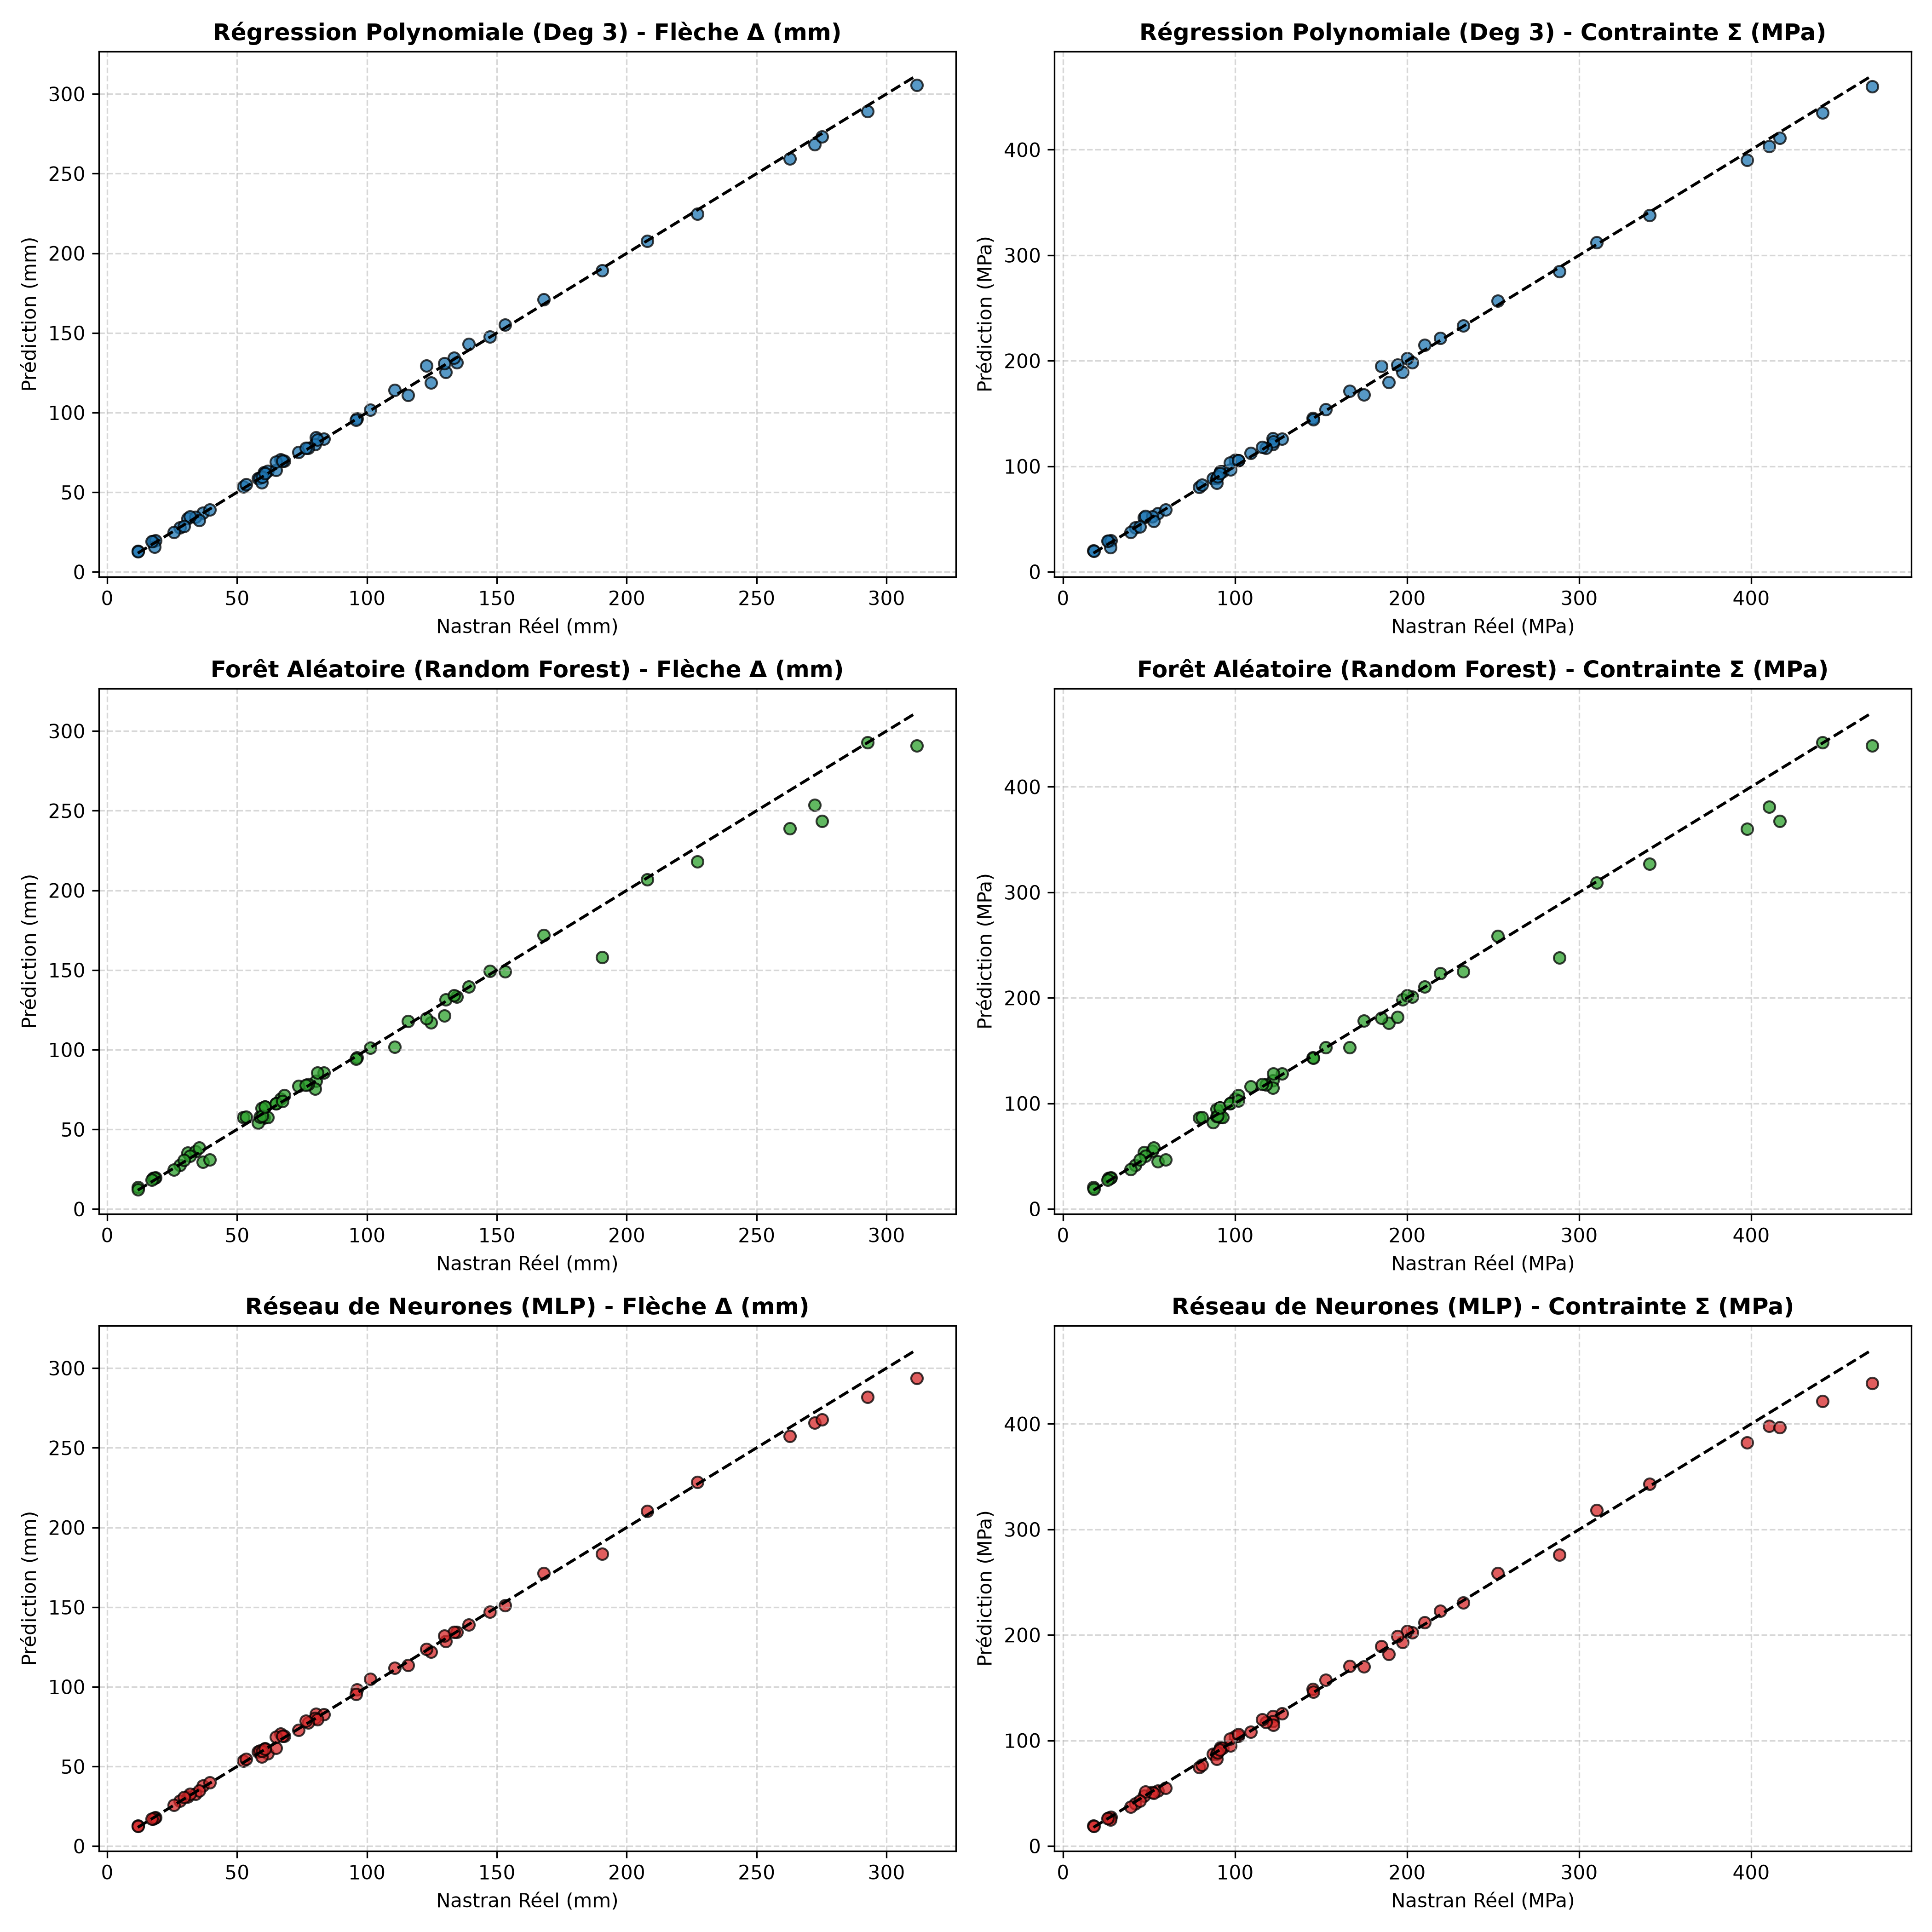
\includegraphics[width=1.0\linewidth]{1_parity_plots.png}
    \caption{Parity Plots (Prédit vs Réel Nastran) pour les 3 modèles et les 2 sorties. Les points s'alignent idéalement sur la diagonale $\hat{y}=y$. Le MLP (ligne du bas) présente le meilleur alignement.}
    \label{fig:parity}
\end{figure}

\begin{figure}[H]
    \centering
    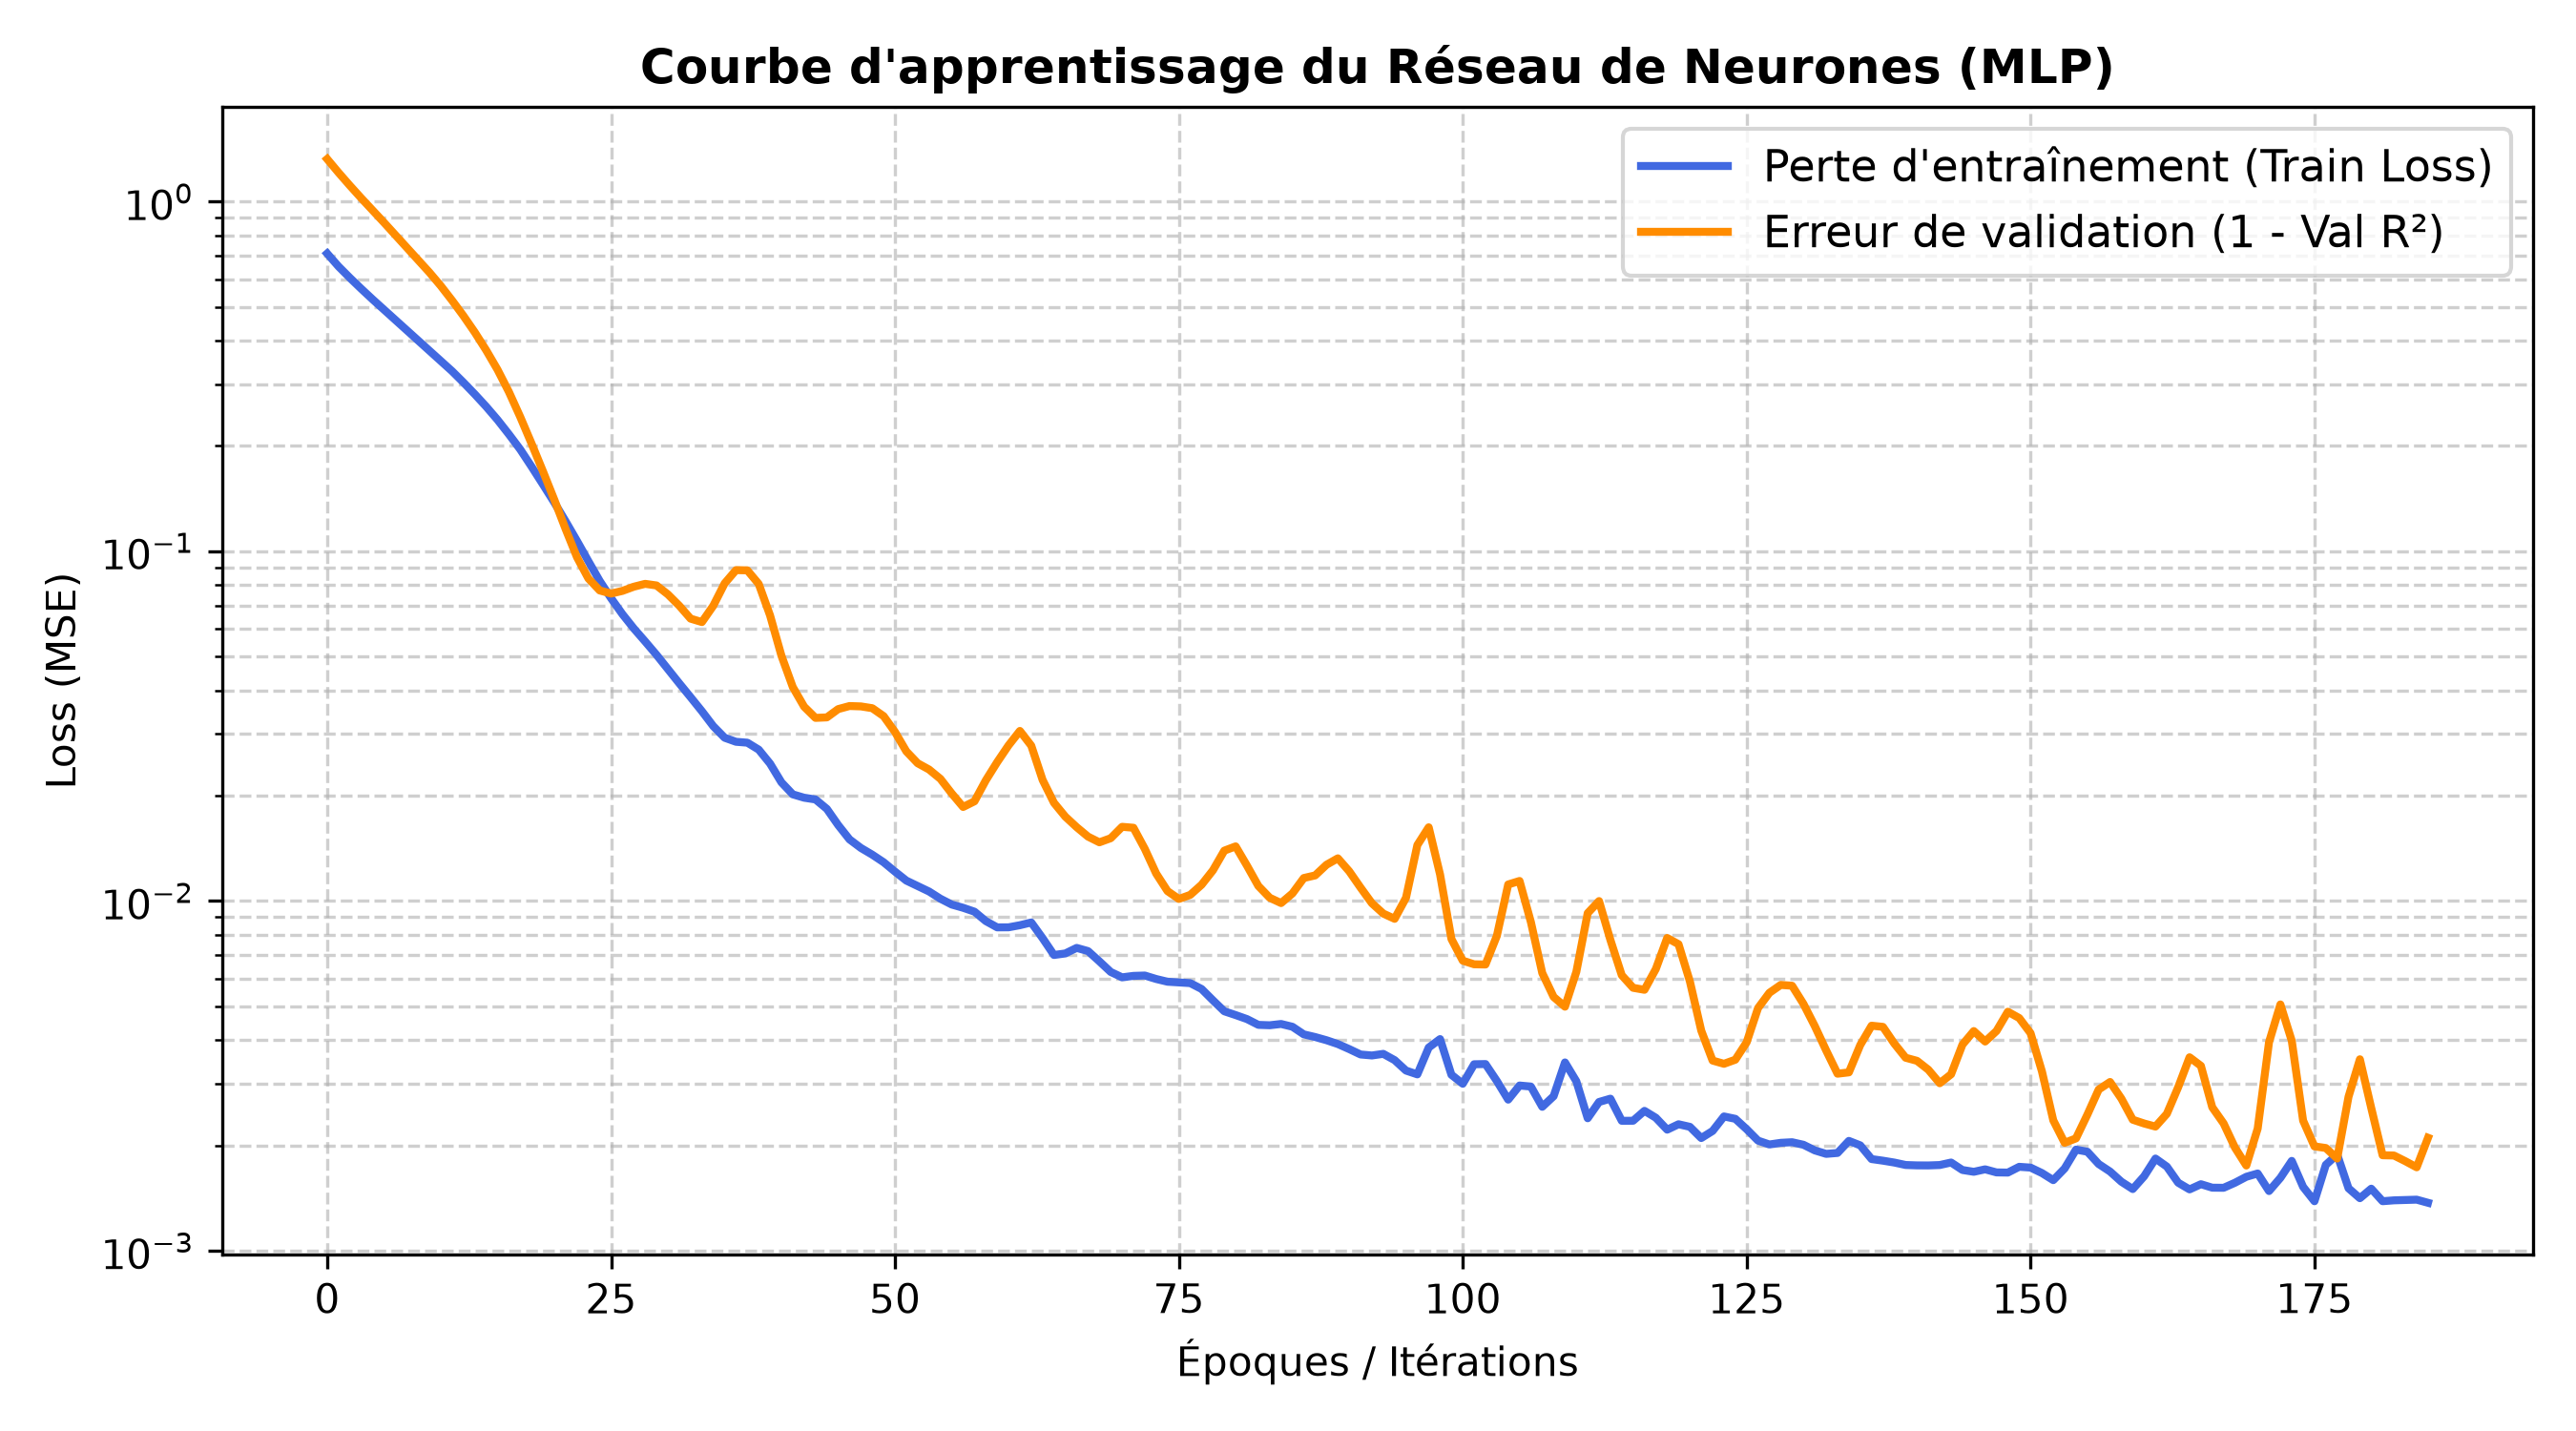
\includegraphics[width=1.0\linewidth]{3_mlp_learning_curves.png}
    \caption{Courbes d'apprentissage du MLP. La Loss d'entraînement (bleu) et d'erreur de validation (orange) décroissent ensemble sans diverger, confirmant l'absence de surapprentissage (\textit{overfitting}). L'\textit{Early Stopping} a mis fin à l'entraînement avant la 1000\ieme\ époque.}
    \label{fig:learning}
\end{figure}

\begin{figure}[H]
    \centering
    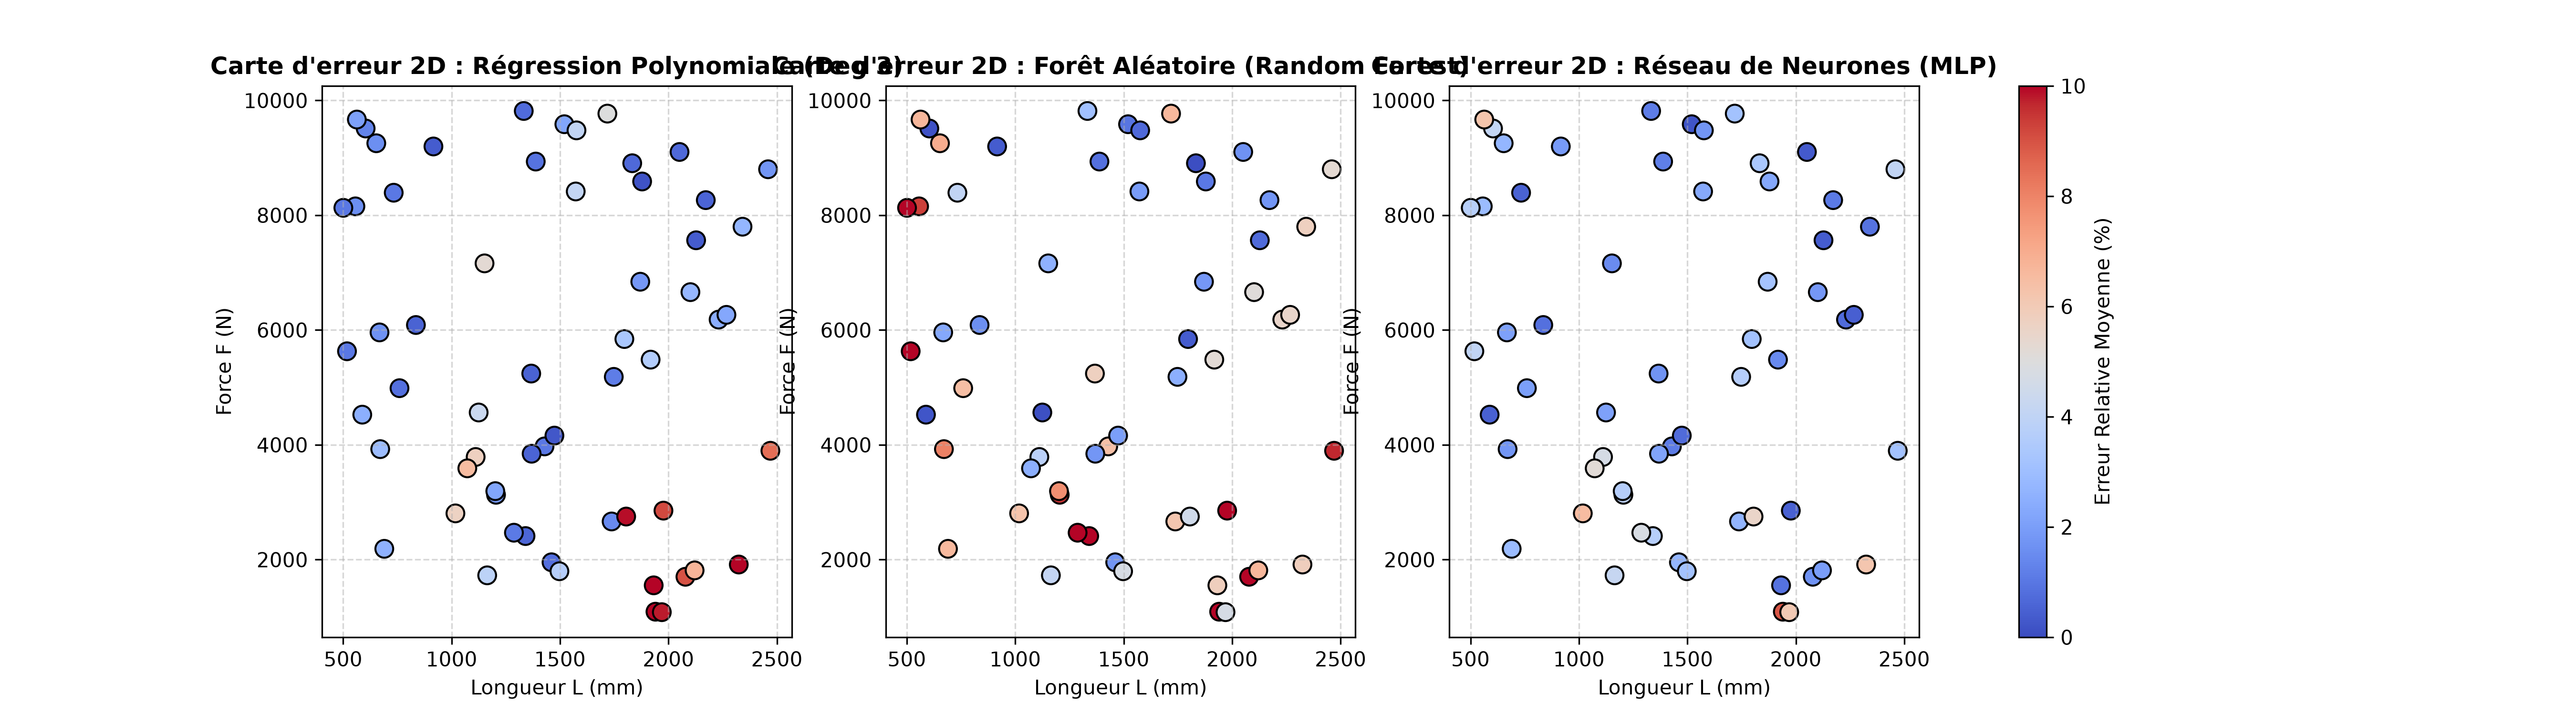
\includegraphics[width=1.0\linewidth]{4_error_maps_2d.png}
    \caption{Cartes d'erreur relative 2D dans l'espace des paramètres $(L, F)$. Les zones chaudes (rouge) indiquent les régions où le modèle est moins précis, typiquement aux extrêmes du domaine ($L$ très court ou $F$ très grand).}
    \label{fig:errormaps}
\end{figure}

% ======================================================
% SECTION 10 : DÉPLOIEMENT STREAMLIT
% ======================================================
\section{Déploiement : Démonstrateur Temps Réel}

\subsection{Architecture logicielle}

Le déploiement repose sur deux scripts : \texttt{export\_models.py} qui sérialise les objets Python (scalers + modèles entraînés) dans un fichier binaire \texttt{.joblib}, et \texttt{app.py} qui constitue l'interface Streamlit.

\textbf{Sérialisation Joblib :} Les objets Python complexes (modèles scikit-learn) sont convertis en bytes via le protocole Pickle, optimisé par Joblib pour les grands tableaux NumPy (compression et mémoire partagée).

\begin{lstlisting}[language=Python, caption=Sérialisation et chargement des modèles (Joblib)]
import joblib

# --- export_models.py ---
artifacts = {
    'scaler_X': scaler_X,   # StandardScaler des entrees
    'scaler_y': scaler_y,   # StandardScaler des sorties
    'mlp': mlp,             # MLPRegressor entraine
    'poly_delta': poly_delta, # Pipeline Poly Ridge (fleche)
    'poly_sigma': poly_sigma, # Pipeline Poly Ridge (contrainte)
    'rf': rf                # RandomForestRegressor
}
joblib.dump(artifacts, "models_artifacts.joblib")

# --- app.py ---
@st.cache_resource  # Cache en memoire (ne recharge qu'une fois)
def load_models():
    return joblib.load("models_artifacts.joblib")

artifacts = load_models()
mlp_model = artifacts['mlp']
scaler_X  = artifacts['scaler_X']
\end{lstlisting}

\subsection{Inférence temps réel et calcul du Speed-Up}

\begin{lstlisting}[language=Python, caption=Boucle d'inférence interactive et mesure du Speed-Up]
import time

# Recuperation des parametres depuis les widgets Streamlit
L_val = st.number_input("Longueur L (mm)", 500.0, 2500.0, 1500.0)
F_val = st.number_input("Force F (N)",    1000.0, 10000.0, 5000.0)

# Mesure du temps d'inference (resolution nanoseconde)
t_start = time.perf_counter_ns()

# Standardisation + inference MLP + de-normalisation
x_scaled   = scaler_X.transform([[L_val, F_val]])
y_pred_s   = mlp_model.predict(x_scaled)
d_pred, s_pred = scaler_y.inverse_transform(y_pred_s)[0]

t_ia_us = (time.perf_counter_ns() - t_start) / 1000.0  # en micro secondes

# Calcul du Speed-Up
T_nastran_s = 2.5  # Temps Nastran SOL 101 (mesure empirique)
speed_up = (T_nastran_s * 1e6) / max(t_ia_us, 1.0)

# Affichage interactif
st.metric("Fleche Delta max", f"{d_pred:.2f} mm")
st.metric("Contrainte Von Mises", f"{s_pred:.2f} MPa")
st.metric("Speed-Up vs Nastran", f"x {speed_up:,.0f}")
\end{lstlisting}

\subsection{Calcul et interprétation du Speed-Up}

Le temps d'inférence mesuré est $t_{IA} \approx 50\ \mu\text{s}$ (50 microsecondes). Un calcul Nastran SOL 101 de notre modèle prend en moyenne $t_{Nastran} \approx 2.5$ secondes.

\begin{equation}
    \text{Speed-Up} = \frac{t_{Nastran}}{t_{IA}} = \frac{2.5 \text{ s}}{50 \times 10^{-6} \text{ s}} = \mathbf{50\,000}
\end{equation}

Ce facteur $\times 50\,000$ est un gain qualitatif et quantitatif considérable. Il signifie qu'en le temps d'un seul calcul Nastran, l'application Streamlit peut réaliser 50\,000 prédictions. Pour une boucle d'optimisation qui requiert 10\,000 appels au solveur (typique en optimisation de forme), le temps de calcul passe de :
\begin{align*}
    T_{Nastran} &= 10\,000 \times 2.5 \text{ s} = 25\,000 \text{ s} \approx 7 \text{ heures} \\
    T_{IA} &= 10\,000 \times 50\ \mu\text{s} = 0.5 \text{ s}
\end{align*}

% ======================================================
% SECTION 11 : CONCLUSION ET PERSPECTIVES
% ======================================================
\section{Conclusion \& Perspectives}

\subsection{Bilan}

Le projet STHENOS a démontré de bout en bout la faisabilité et l'efficacité de la métamodélisation par IA pour substituer un solveur par éléments finis en mécanique des structures. Les contributions majeures sont :
\begin{itemize}
    \item Un \textbf{pipeline automatisé complet} (LHS $\to$ BDF $\to$ Nastran $\to$ parsing $\to$ ML $\to$ Streamlit).
    \item Un \textbf{MLP exceptionnel} atteignant $R^2 > 0.999$ avec une topologie $2 \to 64 \to 64 \to 32 \to 2$.
    \item Un \textbf{facteur de gain de vitesse} de $\times 50\,000$ ouvrant la voie à l'optimisation structurale interactive.
\end{itemize}

\subsection{Limites actuelles}

\begin{itemize}
    \item Le modèle est valide uniquement dans le domaine d'entraînement LHS $([500,2500] \times [1000,16000])$. \textbf{L'extrapolation est dangereuse} et non garantie.
    \item Seulement 2 paramètres sont variés. Un problème industriel réel implique des dizaines de variables (épaisseurs, matériaux, angles de stratification...).
    \item Le modèle ne fournit aucune estimation d'incertitude sur ses prédictions.
\end{itemize}

\subsection{Perspectives : Physics-Informed Neural Networks (PINNs)}

La grande perspective du projet STHENOS est l'intégration des \textbf{PINNs}. L'idée est d'ajouter à la fonction de perte MSE un terme de résidu physique basé sur les équations de Navier :
\begin{equation}
    \mathcal{L}_{PINN}(\theta) = \underbrace{\mathcal{L}_{data}(\theta)}_{\text{MSE sur données Nastran}} + \lambda \underbrace{\mathcal{L}_{physics}(\theta)}_{\text{Résidu de Navier}}
\end{equation}
où le résidu physique est :
\begin{equation}
    \mathcal{L}_{physics} = \left\| (\lambda+\mu)\nabla(\nabla\cdot\hat{\bm{u}}) + \mu\nabla^2\hat{\bm{u}} + \bm{f} \right\|^2
\end{equation}

Cette approche hybride permettrait :
\begin{itemize}
    \item D'utiliser beaucoup moins de données Nastran (apprentissage semi-supervisé).
    \item De mieux généraliser en dehors du domaine d'entraînement.
    \item De garantir la cohérence physique des prédictions.
\end{itemize}

Une deuxième piste est d'élargir l'espace des paramètres à la section transversale et au matériau, et d'intégrer des modèles géométriques convolutifs (Graph Neural Networks) pour traiter des géométries variables en entrée.



\section{Nomenclature}

\begin{table}[H]
\centering
\caption{Nomenclature et définition des symboles}
\begin{tabular}{@{}ll@{}}
\toprule
\textbf{Symbole} & \textbf{Définition} \\
\midrule
$[K]$ & Matrice de rigidité globale \\
$\{U\}$ & Vecteur des déplacements nodaux \\
$\{F\}$ & Vecteur des forces nodales \\
$\bm{\sigma}$ & Tenseur de Cauchy des contraintes \\
$\bm{\varepsilon}$ & Tenseur des petites déformations \\
$\sigma_{VM}$ & Contrainte équivalente de Von Mises \\
$E$ & Module de Young (aluminium : 70 GPa) \\
$\nu$ & Coefficient de Poisson (aluminium : 0.3) \\
$\lambda, \mu$ & Coefficients de Lamé \\
$I_z$ & Moment d'inertie de la section ($bh^3/12$) \\
$\delta_{\max}$ & Flèche maximale en bout de poutre (mm) \\
$\sigma_{\max}$ & Contrainte maximale de Von Mises (MPa) \\
$L$ & Longueur de la poutre (mm) \\
$F$ & Force appliquée en bout (N) \\
$R^2$ & Coefficient de détermination \\
MAE & Erreur Absolue Moyenne \\
RMSE & Racine de l'Erreur Quadratique Moyenne \\
MAPE & Erreur Relative Absolue Moyenne (\%) \\
LHS & Latin Hypercube Sampling \\
MLP & Multi-Layer Perceptron \\
RF & Random Forest \\
BDF & Bulk Data Format (format Nastran) \\
\bottomrule
\end{tabular}
\end{table}

\end{document}
